\documentclass{article}
\usepackage{graphicx} % Required for inserting images
\usepackage{tikz}
\graphicspath{ {./} }

\title{COMPSCI 3N03 Assignment 3}
\author{Aditya Sahni, Karan Sandhu, Ankur Pandey, Manavi Manavi }
\date{March 2025}

\begin{document}

\maketitle

\section*{Detailed Explanation of the Protocol}

\subsection*{Overview}
This report details the communication protocol for a networked ASCII ``Battle Game" implemented in C, consisting of a server (server.c) and a client (client.c). The game supports up to 4 players in a turn-based system, where players can move, attack with shurikens, or quit the game. The server manages the game state, processes client commands, and broadcasts updates to all connected clients. The client sends commands to the server and displays the game state received from the server.
\newline
\newline
The protocol is built on TCP for reliable communication, using a simple text-based message format. Below, we describe the protocol, the recognized commands, the message flow, and provide a sequence diagram to illustrate the client-server interaction.

\subsection*{Connection Establishment}

\begin{enumerate}
    \item Connection Setup
        \begin {itemize}
            \item \textbf{Transport Layer}: The protocol uses TCP for reliable, ordered message delivery.
            \item \textbf{Server Initialization}:
            \begin {itemize}
                \item The server starts by binding to a specified port (e.g., \texttt{./server 3000}) and listens for incoming connections.
                \item It can accept up to 4 clients (\texttt{MAX\_CLIENTS = 4}).
                \item If the server is full, it sends the message \textbf{``Server full. Please try again later."} to the new client and closes the connection.
            \end {itemize}
            \item \textbf{Client Connection}:
            \begin {itemize}
                \item The client connects to the server using the server's IP address and port (e.g., \texttt{./client 127.0.0.1 3000}).
                \item Upon successful connection, the server assigns the client a player ID (0 to 3, corresponding to players A to D) and initializes their position on the grid (e.g., Player A at (0, 0), Player B at (1, 0), etc.).
                \item The server increments its \texttt{clientCount} and logs: "\textbf{New client connected! Connected to ($<$hostname$>$, $<$port$>$). Active clients: $<$count$>$/4}".
            \end {itemize}
    \end {itemize}
    \item Game State
    \begin {itemize}
        \item \textbf{Grid}: A 5x5 ASCII grid (\texttt{GRID\_ROWS = 5, GRID\_COLS = 5})
        \begin {itemize}
            \item \texttt{.} represents an empty cell.
            \item \texttt{\#} represents an obstacle (in our case, at positions (2, 2) and (1, 3)).
            \item \texttt{A, B, C, D} represent players.
            \item \texttt{*} represents a shuriken.
        \end {itemize}
        \item \textbf{Players}:
        \begin {itemize}
            \item Each player has a position (x, y), health points (HP, initially 100), and one shuriken.
            \item Players are identified as A (index 0), B (index 1), C (index 2), and D (index 3).
        \end {itemize}
        \item \textbf{Turn-Based System}:
        \begin {itemize}
            \item The game operates on a turn-based system, starting with Player A (index 0).
            \item The server maintains a \texttt{currentTurn} variable to track whose turn it is.
            \item After each turn, the server rotates the turn to the next active player with HP $>$ 0 using \texttt{rotateTurn()}.
        \end {itemize}
    \end {itemize}
    \item \textbf{Recognized Commands}:
    
        The client sends commands as plain text strings. The server recognizes the following commands:
        \begin{itemize}
            \item \texttt{MOVE $<$DIRECTION$>$}:
                \begin {itemize}
                    \item Format: \texttt{"MOVE UP", "MOVE DOWN", "MOVE LEFT", "MOVE RIGHT"}.
                    \item Action: Moves the player one cell in the specified direction if the move is within bounds and not blocked by an obstacle (\texttt{\#}).
                    \item Example: If Player A is at (0, 0) and sends "MOVE DOWN", they move to (1, 0) if the cell is not an obstacle.
                \end {itemize}
            \item \texttt{ATTACK $<$DIRECTION$>$}:
                \begin {itemize}
                    \item Format: \texttt{"ATTACK UP", "ATTACK DOWN", "ATTACK LEFT", "ATTACK RIGHT"}.
                    \item Action: Launches a shuriken in the specified direction from the player's position.
                    \begin {itemize}
                        \item The shuriken spawns one cell away in the direction of the attack (e.g., if Player A at (0, 0) sends \texttt{"ATTACK DOWN"}, the shuriken spawns at (1, 0)).
                        \item If the spawn position is valid (within bounds and not an obstacle), the shuriken becomes active and moves one cell per turn in the same direction.
                        \item If the shuriken hits a player (i.e., occupies the same cell), it deals 50 damage and deactivates.
                        \item If the shuriken hits a wall (\texttt{\#}) or goes out of bounds, it deactivates.
                    \end {itemize}
                    \item Example: If Player A at (0, 0) sends "ATTACK DOWN" and Player B is at (1, 0), Player B takes 50 damage (HP: 100 → 50).
                \end {itemize}
            \item \texttt{QUIT}:
                \begin{itemize}
                    \item Format: \texttt{"QUIT"}.
                    \item Action: The player quits the game, their state is reset, and their socket is closed.
                    \item Example: If Player A sends \texttt{"QUIT"}, they are removed from the game, and other players are notified.
                \end{itemize}
            \end{itemize}
    \item Server Responses and Messages:

        The server sends the following messages to the clients:
        \begin {itemize}
            \item \textbf{Game State Update}:
                \begin{itemize}
                    \item Format:
\begin{verbatim}
STATE:

<grid row 1>
<grid row 2>
<grid row 3>
<grid row 4>
<grid row 5>

ACTIVE PLAYER INFO (IF EXISTS)
Player <ID>
Player position: (<x>, <y>)
Player health points <HP>
...
\end{verbatim}
                \item Sent: After every command (via \texttt{broadcastState()}), when a player connects, disconnects, or quits.
                \item Example:
\begin{verbatim}
STATE:

A....
B...#
..#..
.....
.....

ACTIVE PLAYER INFO (IF EXISTS)
Player 0
Player position: (0, 0)
Player health points 100
Player 1
Player position: (1, 0)
Player health points 100
\end{verbatim}
            \end{itemize}
            \item \textbf{Turn Notifications}:
                \begin{itemize}
                    \item To the current player: ``\textbf{It's your turn, Player X}" (e.g., ``\textbf{It's your turn, Player A}").
                    \item To other players: ``\textbf{It's Player X's turn}" (e.g. ``\textbf{It's Player A's turn}").
                    \item Sent: After every turn rotation (via \texttt{rotateTurn()}).
                \end{itemize}
            \item \textbf{Not Your Turn}:
                \begin{itemize}
                    \item Message: ``\textbf{Sorry, it's not your turn}".
                    \item Sent: If a player sends a command when it's not their turn.
                \end{itemize}
            \item \textbf{Shuriken Hit}:
                \begin{itemize}
                    \item The server logs: ``\textbf{Player X hit by shuriken! HP reduced to Y}", but this is not sent to clients.
                    \item The updated HP is reflected in the game state broadcast.
                \end{itemize}
            \item \textbf{Player Defeated}:
                \begin{itemize}
                    \item To the defeated player: ``\textbf{You have died!}".
                    \item Sent: When a player's HP drops to 0 or below (via \texttt{checkShurikenCollision()}).
                    \item The server logs: ``\textbf{Player X has been defeated!}''.
                \end{itemize}
            \item \textbf{Player Quit}:
                \begin{itemize}
                    \item To the quitting player: ``\textbf{You have quit the game.}''.
                    \item To other players: ``\textbf{Player X has quit the game.}".
                    \item Sent: When a player sends ``\texttt{QUIT}".
                \end{itemize}
            \item \textbf{Player Disconnected}:
                \begin{itemize}
                    \item To other players: ``\textbf{Player X has disconnected.}".
                    \item Sent: When a player disconnects unexpectedly (e.g., closes their client).
                \end{itemize}
        \end{itemize}
    \item Message Flow
    
    The message flow follows a turn-based pattern:
    \begin{enumerate}
        \item Client Connects:
            \begin{itemize}
                \item Client connects to the server.
                \item Server assigns a player ID, initializes the player's state, and broadcasts the updated game state to all clients.
                \item If the client is the first player (Player A), the server sends: ``\textbf{It's your turn, Player A}".
            \end{itemize}
        \item Turn-Based Command Processing:
            \begin{itemize}
                \item The client whose turn it is sends a command (e.g., \texttt{"MOVE DOWN", "ATTACK RIGHT", "QUIT"}).
                \item If it's not the client's turn, the server responds with "\textbf{Sorry, it's not your turn}".
                \item Otherwise, the server processes the command:
                    \begin{itemize}
                        \item Updates the game state (e.g., moves the player, launches a shuriken, or removes the player if they quit).
                        \item Broadcasts the updated game state to all clients.
                        \item Rotates the turn and sends turn notifications.
                    \end{itemize}
            \end{itemize}
        \item Shuriken Movement:
            \begin{itemize}
                \item At the start of each turn, the server moves all active shurikens and checks for collisions.
                \item If a shuriken hits a player, their HP is reduced, and the updated state is broadcast.
            \end{itemize}
        \item Disconnection:
            \begin{itemize}
                \item If a client sends ``\texttt{QUIT}" or disconnects unexpectedly, the server resets their state, notifies other players, and broadcasts the updated state.
            \end{itemize}
    \end{enumerate}
\end{enumerate}
\section*{Sequence Diagram}
Below is a sequence diagram illustrating the communication between two clients (Client A and Client B) and the server during a game session. The diagram includes connection, command processing, shuriken hits, and disconnection.
\begin{figure}[h]
    \centering
    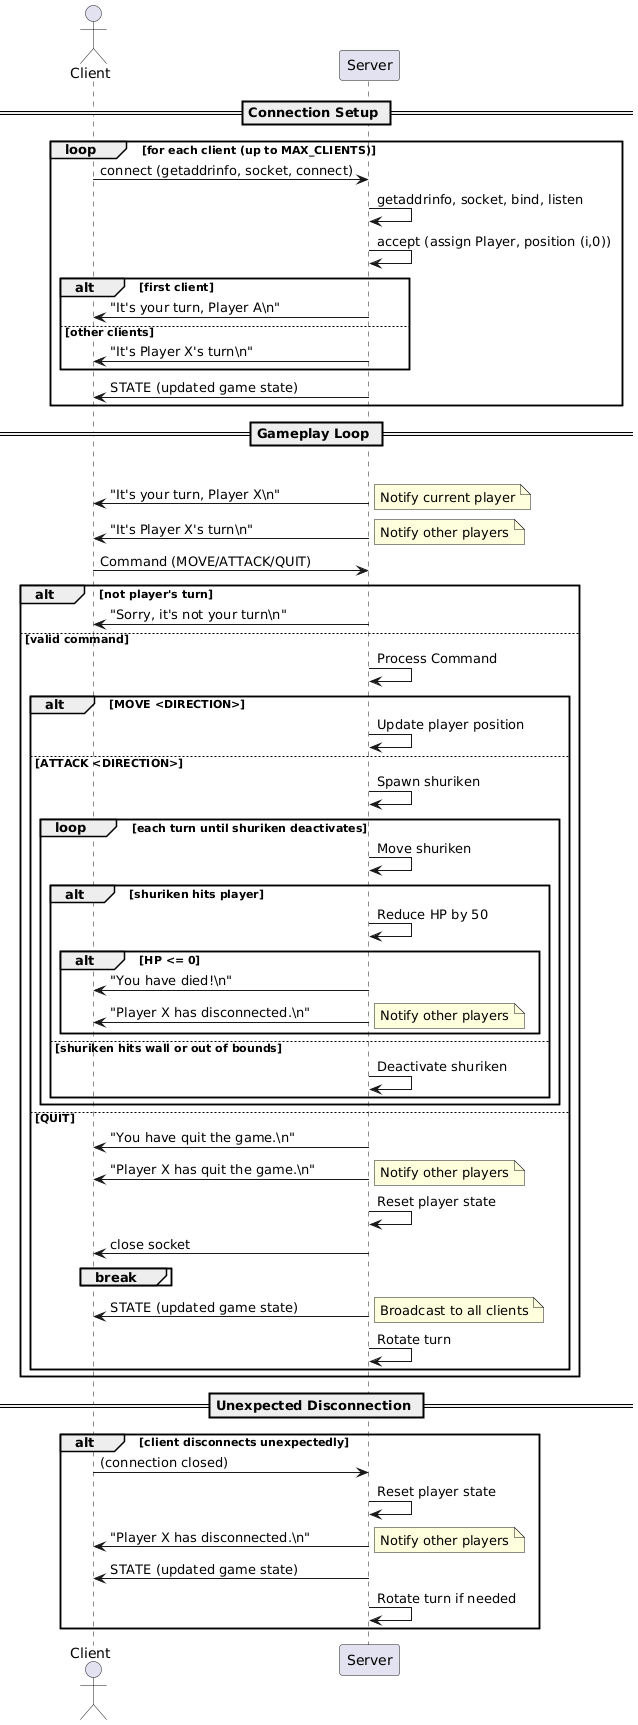
\includegraphics[width=8cm, height=20cm]{sequence_diagram.png}
    \label{fig:sequence}
\end{figure}
\clearpage
\section*{Final Protocol Summary}
The networked ASCII Battle Game protocol defines a set of commands and server messages to facilitate turn-based gameplay. Players can issue commands such as \texttt{MOVE $<$DIRECTION$>$} to move their character in the specified direction (\texttt{UP, DOWN, LEFT, RIGHT}), \texttt{ATTACK $<$DIRECTION$>$} to launch a shuriken in the chosen direction (\texttt{UP, DOWN, LEFT, RIGHT}), and \texttt{QUIT} to exit the game, which removes the player from the session. 
\newline
\newline
The server communicates with clients through various messages, including the game state, formatted as ``STATE: $\backslash$n $<$grid$>$ $\backslash$n ACTIVE PLAYER INFO (IF EXIST) $\backslash$n $<$player info$>$", which provides the current grid and player details. 
\newline
\newline
Turn notifications are sent to inform the current player with ``\textbf{It's your turn, Player}" and other players with ``\textbf{It's Player X's turn}", while an error message, ``\textbf{Sorry, it's not your turn}", is sent if a player attempts an action out of turn. 
\newline
\newline
When a player's HP drops to zero, the server sends ``\textbf{You have die}" to the affected player. For the \texttt{QUIT} command, the quitting player receives ``\textbf{You have quit the game}", and other players are notified with ``\textbf{Player X has quit the game}". If a player disconnects unexpectedly, the server broadcasts ``\textbf{Player X has disconnected}" to the remaining players.
\newline
\newline
The message flow of the protocol follows a structured sequence to ensure smooth gameplay. When a client connects, the server assigns a player ID and broadcasts the updated game state to all clients. The game then enters a turn-based loop where the server notifies the current player of their turn, prompting them to send a command, which the server processes before broadcasting the updated state and rotating the turn to the next player. At the start of each turn, the server handles shuriken movement and collision checks, updating the game state accordingly. If a client disconnects, either by sending \texttt{QUIT} or unexpectedly, the server resets the player's state, broadcasts the updated state to all remaining clients, and continues the game. This flow ensures a fair and consistent multiplayer experience.
\subsection*{Additional Features}
Here are some additional features we've introduced. We won't go into detail here, as we've already explained them previously.
\begin{itemize}
    \item \textbf{Shuriken}: Added a shuriken mechanic, allowing players to attack in a specified direction, dealing 50 damage on hit.
    \item \textbf{Turn-by-Turn Gameplay}: Implemented a turn-based system, ensuring fair play by rotating turns among active players.
    \item \textbf{Proper QUIT Mechanics}: Enhanced the QUIT command to notify all players, reset the quitter's state, and close their socket cleanly.
    \item \textbf{Border Adherence}: Fixed movement to prevent players from going out of the 5x5 grid, ensuring valid moves within boundaries.
\end{itemize}
\end{document}
